\documentclass[preprint,3p]{elsarticle}
%\documentclass[preprint]{aastex}
\usepackage{aas_macros}
\usepackage{amsmath,amssymb}
\usepackage{mathrsfs}
\usepackage{graphicx}
\usepackage{bm}
\usepackage{hyperref}
\DeclareMathOperator\erf{erf}
\newcommand{\mli}[1]{\mathit{#1}}
%\usepackage{epstopdf}


\begin{document}

%\begin{frontmatter}
%
%\title{Toy Model}
%\author{A.~G. Kim\corref{cor1}}
%\ead{agkim@lbl.gov}
%\address{Physics Division, Lawrence Berkeley National Laboratory, 1 Cyclotron Road, Berkeley CA, USA 94720}
%
%\begin{abstract}
%\end{abstract}
%\begin{keyword}
%\end{keyword}
%\end{frontmatter}

\section{Likelihood}
\label{likelihood:sec}

The ambition is to construct a model to determine the likelihood of DES-like
supernova data.
The conceptual structure of the model is shown in Figure~\ref{pgm:fig}. 
\begin{figure}[htbp] %  figure placement: here, top, bottom, or page
   \centering
   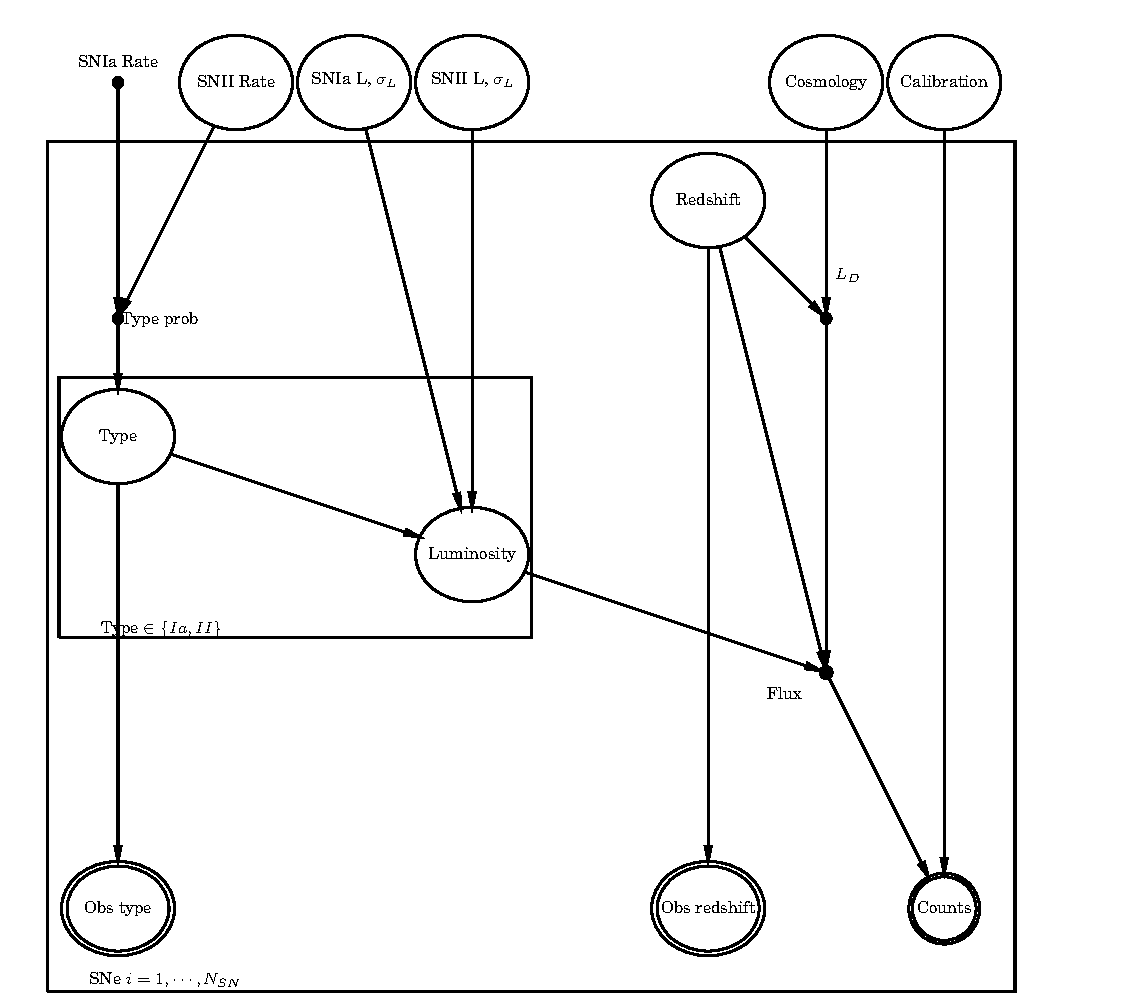
\includegraphics[width=6.5in]{../results//nodes_pgm.pdf} 
   \caption{Probabilistic Graphical Model for the SN~Ia analysis.  
   \label{pgm:fig}}
\end{figure}

In the toy model there are three types of data that
may be observed for each supernova:
\begin{itemize}
\item $c_o$: Counts at peak brightness.
\item $z_o$: Redshift.
\item $T_o$: Transient type.
\end{itemize}

There are selection criteria $S_c$ and $S_T$ for the inclusion of an object in the
sample and for a successul typing.
In what follows we assume that the typed objects are drawn from the same underlying
distribution as the sample $S_c=S_T$, and that the selection criterion is a brightness
threshold $S_c = c_o \ge c_T$.  (The spectroscopic sample $S_T$ 
eventually should depend on the
photometry and the quality of the spectroscopic data.)

For this preliminary discussion the top-level parameters are denoted by $X$,
latent parameters $L$ and $T$.  

It is useful to split the data into two cases depending on whether or not
the transient has a type measurement $T_o$.

\subsection{Case Typed}
For Case Typed the likelihood is
\begin{align}
\mathcal{L}(T_o,z_o,c_o | S_c, S_T, z, X) & =  \int dL \sum_i p(T_o,z_o,c_o | T_i, L, S_c, S_T, z, X) p(L |  T_i,  S_c, S_T, z, X) P(T_i|S_c, S_T, z, X).
\end{align}
We assume that the observations give a perfect measurement of type and redshift,
so that
\begin{align}
p(T_o|T) & =\delta(T_o-T)\\
p(z_o|z) & =\delta(z_o-z);
\end{align}
practically $T$ and $z$ are no longer probabilistic but are fixed.
Then
\begin{align}
\mathcal{L}(T_o,z_o,c_o | S_c, S_T, z, X) & =  \int dL p(c_o | T=T_o, L, S_c, S_T, z=z_o, X) p(L| T=T_o, S_c, S_T, z=z_o, X)  P(T_o|S_c, S_T, z=z_o, X) \\
&= \int dL \frac{ p(c_o, S_c, S_T | T=T_o, L, z=z_o, X) }{P(S_c, S_T, | T=T_o, L,  z=z_o, X) }
\frac{p(L, S_c, S_T | T=T_o, z=z_o, X)}{P(S_c, S_T| T=T_o,  z=z_o, X)}
\frac{p(T_o, S_c, S_T | z=z_o, X)}{P(S_c, S_T| z=z_o, X)} \\
&= \frac{\int dL p(L|T_o, z=z_o, X) P(T_o|z=z_o, X) p(c_o, S_c, S_T | T=T_o, L, z=z_o, X)}{P(S_c, S_T| z=z_o, X)}
\end{align}

The normalization term is determined by
\begin{align}
P(S_c, S_T| z=z_o, X) & =\sum_i \int_{-\infty}^{\infty} dc_o \mathcal{L}(T_i,z_o,c_o | S_c, S_T, z, X) \\
& = \sum_i \int_{c_T}^{\infty} dc_o \mathcal{L}(T_i,z_o,c_o | S_c, S_T, z, X)\\
& = \sum_i  P(T_i|z=z_o, X)\int dL p(L|T_i, z=z_o, X)  \left[\int_{c_T}^{\infty} dc_o  p(c_o | T=T_i, L, z=z_o, X)\right]
\end{align}
as $p(c_o | T=T_o, L, z)=0$ when $c_o < c_T$.

\subsection{Case Not Typed}


For Case Not Typed the likelihood is
\begin{align}
\mathcal{L}(z_o,c_o | S_c, S_T, z, X) & =  \int dL \sum_i p(z_o,c_o | T_i, L, S_c, S_T, z, X) p(L |  T_i,  S_c, S_T, z, X) P(T_i|S_c, S_T, z, X).
\end{align}

For the redshift measurement, we take a set of potential host galaxies, where galaxy $j$
are redshift $z_j$ has probability $p_j$ of being the host
\begin{equation}
p(z_o|S_c, S_T, z, X) = \sum_j p_j\delta(z_j-z).
\end{equation}
Then
\begin{align}
\mathcal{L}(z_o,c_o | S_c, z, X) & =  \sum_j p_j \int dL \sum_{i} p(c_o | T_i, L, S_c, z=z_j, X) p(L |  T_i,  S_c,  z=z_j, X) P(T_i|S_c, z=z_j, X) \\
&=  \frac{\sum_j p_j \int dL p(c_o, S_c | L, z=z_j, X) \sum_{i}  p(L|T_i, z=z_j, X) P(T_i|z=z_j, X)   }{P(S_c| z=z_j, X)},
\end{align}
where we use the fact that the counts do not directly depend on type.

The normalization term is
\begin{align}
P(S_c| z=z_o, X) & = \int_{c_T}^{\infty} dc_o \mathcal{L}(T_i,z_o,c_o | S_c, S_T, z, X)\\
& =  \sum_j p_j  \sum_{i} P(T_i|z=z_j, X)  \int dL  p(L|T_i, z=z_j, X) 
\left[ \int_{c_T}^\infty dc_o p(c_o| T=T_i, L, z=z_j, X) \right].
\end{align}



\section{Model}
\label{model:sec}

We now go into more detail into the model and the form of the pdf's that enter
into the likelihoods described in \S\ref{likelihood:sec}.

A description of the nodes follow.  Numbers are illustrative. 

\subsection{Cosmology}
The Flat $w$CDM cosmology.

\begin{align}
\Omega_M & \sim \ln{\mathcal{N}}(\ln{0.28},0.1)\\
w_0 & \sim \mathcal{N}(-1,0.05)
\end{align}

\subsection{Calibration}
Photometric zeropoints for each band.
\begin{equation}
Z \sim \mathcal{N}(0,0.02)
\end{equation}

\subsection{SNIa Rate}
Type~Ia SN rate. In the analysis only relative rates between different transients are important.
We take the rates relative to the SN~Ia rate
\begin{equation}
r_{SNIa} = 1.
\end{equation}

\subsection{SNII Rate}
Type~II SN rate, relative to the SN~Ia rate
\begin{equation}
r_{SNII} \sim \mathcal{U}(0.25, 4).
\end{equation}

\subsection{SNIa Luminosity}
The mean luminosity and intrinsic dispersion for SNe~Ia. In fact work with log-luminosity, intrinsic
dispersion in mag units.
\begin{align}
\ln{L}_{SNIa} & \sim \mathcal{N}(\ln{1}, 0.02) \\
\sigma_{SNIa} & \sim \ln{\mathcal{N}}(\ln{0.1},0.1).
\end{align}

\subsection{SNII Luminosity}
The mean luminosity and intrinsic dispersion for SNe~II. In fact work with log-luminosity, intrinsic
dispersion in mag units.
\begin{align}
\ln{L}_{SNII} & \sim \mathcal{N}(\ln{0.5}, 0.02) \\
\sigma_{SNII} & \sim \ln{\mathcal{N}}(\ln{0.4},0.1).
\end{align}

\subsection{SNIa~Probability}
Probability an object is SN~Ia
\begin{align}
p_{SNIa} &= \frac{r_{SNIa}}{r_{SNIa}+r_{SNII}} \nonumber \\
p_{SNII}&=1-p_{SNIa}.
\label{prob:eqn}
\end{align}
\subsection{Type}
The type of the object $T$ is drawn from the Bernoulli distribution 
\begin{equation}
T | p_{SNIa} \sim \mathcal{B}(1-p_{SNIa}),
\end{equation}
with the convention that $T=0$ corresponds to SN~Ia.

The type probability appears explicitly in the calculation of the likelihoods.
\begin{align}
P(T_{SNIa} | z=z_j, X) &= p_{SNIa}\\
P(T_{SNII} | z=z_j, X) &= p_{SNII}
\end{align}
\subsection{Observed Type}
The observed type is assumed to be perfect.
\begin{equation}
T_o = T.
\end{equation}

\subsection{Luminosity}
For our model
\begin{equation}
\ln{L} | T, \ln{L}_{T},\sigma_{T} \sim \mathcal{N}\left( \ln{L}_{T},\frac{\ln{10}}{2.5}\sigma_{T}\right).
\end{equation}

The corresponding pdf appears in the likelihood.

\subsection{Redshift}
The redshift is drawn from a flat distribution
\begin{equation}
z\sim \mathcal{U}(0,\infty).
\end{equation}
%
%\subsection{Neighbor Galaxy Redshifts}
%Each neighbor redshift is drawn from a flat distribution.  The redshift for neighbor
%$i$ is  
%\begin{equation}
%z_{N,i} \sim \mathcal{U}(0,\infty).
%\end{equation}

\subsection{Observed Redshift}
In our model the measured redshift is a sum of delta functions
\begin{equation}
p(z_o|z) = \sum_i p_i \delta(z-z_i),
\end{equation}
where galaxy $i$ at
redshift $z_i$ has probability $p_i$ of being
the host.  

\subsection{Counts}
The luminosity distance comes from the physics-theory function
\begin{equation}
d_L = d_L(z; \Omega_M, w0),
\end{equation}
the flux is
\begin{equation}
f = \frac{L}{4\pi d_L^2},
\end{equation}
and expected counts is
\begin{equation}
c_\star = 10^{Z/2.5}f.
\end{equation}
The distribution of counts for all transients is 
\begin{equation}
c_o | c_\star, \sigma_c \sim \mathcal{N}(c_\star, \sigma_c),
\end{equation}
where $\sigma_c$ is the measurement noise.

\subsection{Sample Selection Normalization}
Anticipating the use of available statistical packages, the likelihoods have been constructed
from standard distribution functions.  The truncated distributions from sample selection
are accounted by the normalization 
terms $P(S_c, S_T| z=z_o, X)$, $P(S_c| z=z_o, X)$.  Although they do not appear
in the PGM, they are treated as nodes who contribute 
$-\ln{P(S_c, S_T| z=z_o, X)}$ to the log-likelihood, where the negative sign reflects that this is a normalization
factor.

\subsection{Implementation Notes}
The following integral appears in the normalization
\begin{equation}
\int dL p(L|T_i, z=z_o, X)  \left[\int_{c_T}^{\infty} dc_o  p(c_o | T=T_i, L, z=z_o, X)\right].
\end{equation}
We actually work with $\ln{L_X}$ and $\sigma_X$.  Setting
\begin{equation}
n=\frac{\ln{L}-\ln{L_X}}{\sigma_X}
\end{equation}
the integral becomes
 \begin{equation}
\sigma_X \int dn p(n\sigma_X + \ln{L_X} |T_i, z=z_o, X)  \left[\int_{c_T}^{\infty} dc_o  p(c_o | T=T_i, L_Xe^{n\sigma_X}, z=z_o, X)\right].
\end{equation}
The two probability distributions are normal so that this reduces to
 \begin{equation}
\frac{1}{2\sqrt{2\pi}} \int dn\, e^{-0.5n^2} \left(1-erf\left(\frac{(c_T - c_\star)}{\sqrt{2}\sigma_c}\right)\right),
\end{equation}
where
\begin{equation}
c_\star = \frac{e^{\ln{L_X}+n\sigma_X}}{4\pi d_L^2}10^{Z/2.5}.
\end{equation}
\end{document}